\documentclass[twoside]{article}

\input{settings/packages}
\input{settings/environments}

\definecolor{ugrey}{HTML}{666666}
\definecolor{ured}{rgb}{0.86, 0.08, 0.24}
\definecolor{ured60}{rgb}{0.916, 0.448, 0.544}
\definecolor{ublue}{rgb}{0.12, 0.56, 1.0}
\definecolor{uhole}{rgb}{0.75, 0.75, 0.75}
% \definecolor{ublue}{HTML}{08088A}
% \definecolor{linkcolor}{HTML}{0000CC}
% \definecolor{urlcolor}{HTML}{006600}
% \hypersetup{
%     pdfstartview=FitH,  
%     linkcolor=linkcolor,
%     urlcolor=urlcolor, 
%     colorlinks=true,
%     citecolor=blue}
% базовая подстройка
\renewcommand{\d}{\, d}
\renewcommand{\leq}{\leqslant}
\renewcommand{\geq}{\geqslant}

\newcommand{\vc}[1]{\boldsymbol{#1}}
\newcommand{\1}{\mathbbm{1}}
\newcommand{\T}{^{\textnormal{T}}}
\newcommand{\D}{^{\dag}}
\newcommand{\sub}[2]{#1_{\textnormal{#2}}}
\newcommand{\vp}{\vphantom{\dfrac{1}{2}}}
\newcommand{\hc}{\mathrm{h.c.}}

\renewcommand{\Im}{\mathop{\mathrm{Im}}\nolimits}
\renewcommand{\Re}{\mathop{\mathrm{Re}}\nolimits}
\newcommand{\diag}{\mathop{\mathrm{diag}}\nolimits}
\newcommand{\std}{\mathop{\mathrm{std}}\nolimits}
\newcommand{\mean}{\mathop{\mathrm{mean}}\nolimits}
\newcommand{\sigmoid}{\mathop{\mathrm{sigmoid}}\nolimits}
\newcommand{\card}{\mathop{\mathrm{card}}\nolimits}
\newcommand{\grad}{\mathop{\mathrm{grad}}\nolimits}
\renewcommand{\div}{\mathop{\mathrm{div}}\nolimits}
\newcommand{\rot}{\mathop{\mathrm{rot}}\nolimits}
\newcommand{\Ker}{\mathop{\mathrm{ker}}\nolimits}
\newcommand{\spec}{\mathop{\mathrm{spec}}\nolimits}
\newcommand{\sign}{\mathop{\mathrm{sign}}\nolimits}
\newcommand{\tr}{\mathop{\mathrm{tr}}\nolimits}
\newcommand{\rg}{\mathop{\mathrm{rg}}\nolimits}
\newcommand{\const}{\textnormal{const}}

\newcommand{\grey}[1]{\textcolor{ugrey}{#1}}
\newcommand{\red}[1]{\textcolor{red}{#1}}
\newcommand{\green}[1]{\textcolor{urlcolor}{#1}}
\newcommand{\blue}[1]{\textcolor{ublue}{#1}}

\newcommand{\cmark}{\text{\ding{51}}}
\newcommand{\xmark}{\text{\ding{55}}}

\newcommand{\addletter}[2]{\begin{picture}(7,7) \put(0,#1){{#2)}} \end{picture}}

\newcommand{\ket}[1]{\left| #1 \right\rangle}
\newcommand{\bra}[1]{\left\langle #1 \right|}

\DeclareDocumentCommand{\bk}{m o m}{
    \IfNoValueTF{#2}{\langle #1 | #3 \rangle}{\langle #1 | #2 | #3 \rangle}
}
\newcommand{\kb}[2]{| #1 \rangle \langle #2 |}

\newcommand{\tth}{\sub{t}{th}}
% add page header

% \pagestyle{fancy}
% \fancyhf{}
% \fancyhead[RE,LO]{\thepage}
% \fancyhead[LE,RO]{Ж\raisebox{-1.5pt}{и}К}
% \fancyhead[CO,CE]{\leftmark}
% \fancyfoot[LE,RO]{\thepage}


\input{settings/symbols}

\begin{document}

\input{settings/set}




% !TEX root = ../master-thesis.tex

% document's head

\begin{center}
    % \LARGE \textsc{Fermionic State Preparation and Imaging \\ in Optical Tweezer Array}
    \LARGE \textsc{Tools for 2D Fermi-Hubbard Simulation: \\ State Preparation and Spin-Resolved Imaging}
\end{center}

\hrule

\phantom{42}

\begin{flushright}
    \begin{tabular}{rr}
        % \textbf{Author}: 
        & Khoruzhii Kirill \\
        % & \\
    % date:
        % \textbf{Date}:
        & \textit{Munich, \today}\\
    \end{tabular}
\end{flushright}

\noindent
Quantum simulation with ultracold atoms requires both high-fidelity preparation of the initial many-body state and site-resolved measurement of the final state. This thesis presents the development of experimental techniques for spin-resolved free-space imaging and deterministic, spin-selective preparation of ultracold fermionic $^6$Li atoms in a two-dimensional optical tweezer array. The array is generated using crossed acousto-optic deflectors, with precise control achieved through a combination of direct camera-based calibration and atom-based feedback. A novel spilling method enables the preparation of arbitrary spin- and site-resolved occupation patterns. The thesis also introduces numerical tools for simulating Fermi-Hubbard dynamics in small systems, laying the groundwork for future out-of-equilibrium quantum simulation experiments.







\thispagestyle{empty}

\newpage

\thispagestyle{empty}

\tableofcontents

% \vfill

% Базовая структура диплома:
% \begin{enumerate*}
%     \item deterministic state preparation (single tweezer)
%     \begin{enumerate*}
%         \item loading (2D MOT, MOT, Dipol Trap, Tweezer)
%         \item spilling
%     \end{enumerate*}
%     \item single-atom spin resolved free space imaging
%     \begin{enumerate*}
%         \item ! flashing and model
%         \item ! image processing
%     \end{enumerate*}
%     \item deterministic state preparation (tweezer array)
%     \begin{enumerate*}
%         \item ! generating
%         \item ! control
%         \item ! balancing
%     \end{enumerate*}
% \end{enumerate*}

% Это история про то как сделать и сфотографировать спиновое состояние в твизере.   

% Нужно выписать contributions! И им следовать.   




\newpage


 
Ещё было бы здорово добавить картинки

\begin{itemize}
	\item Демонстрация с Random Unitaries (Xinyi тезис)
	\item Схема установки, фото 3D mot
	\item BEC
	\item ? Feshbach resonance
	\item Imaging: Эксперимент. Alternating beams (с осциллографа), разница двух облачков (один, два continous, два alternating)
	\item Imaging: histogram noise vs atoms, raw nuvu img
	\item MWM (simulation, ? observed)
	\item Flashing. Экспериментальная установка, табличка с её параметрами
	\item State preparation: spilling. Схематичное изображение (посмотреть в Heidelberg thesis). Step plot. 
	\item State preparation: схема подготовки site- and spin- resolved состояния.
	\item Стабилизация: итерации стабилизации для single-value feedback
	\item Theory: описание fermi-hubbard, фазовая диаграмма (посмотреть coepsill)
	\item Theory: термализация vs локализация для решётки 8x8
	\item Theory: вклад от лабиринтов в локализацию
	\item Tweezer Array. Схема AOD, crosstalk basics
\end{itemize}



\section{Single-atom spin resolved free space imaging}

\subsection{Experimental setup}
\red{Здесь схема оптики для подготовки лучей в preparation board и схема лучей и подключения для main board}.

\begin{figure}
    \centering
    \addletter{140}{a}
    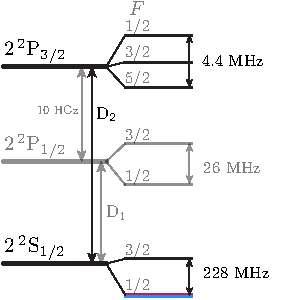
\includegraphics{fig-ai/li-levels-base.pdf}
    \hfill
    \addletter{140}{b}
    \includegraphics{fig-py/li6-zeeman.pdf}
    \hfill
    \addletter{140}{c}
    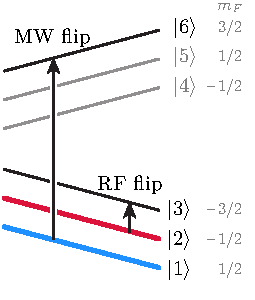
\includegraphics{fig-ai/li-levels.pdf}
    \caption{
        \textbf{${}^6$Li energy levels}. 
        a) Level diagram of the ground and 2P excited states of ${}^6$Li \cite{gehm_preparation_2003}. 
        b) Zeeman splitting of the hyperfine levels of the $2\, {}^2\mathrm{S}_{1/2}$ state in ${}^6$Li \cite{serwane_deterministic_2011, sibalic_arc_2017}. With dashed line was marked non-interacting regime for 1-2 mixture at 527 Gs. c) As different spin states for physics we consider state $\ket{1}$ and $\ket{2}$, but for imaging it is worth to flip them to close transitions.
        \red{Можно разделить (b), чтобы показать и расщепление для P32.}
    }
    \label{fig:li6levels}
\end{figure}

\subsection{SSH Model}
Исходно SSH model выглядит как
\begin{equation*}
	H = t_1 \sum_n \kb{n,B}{n,A} + t_2 \sum_n \kb{n+1, A}{n, B} + \hc
\end{equation*}
что в нашем случае переписывается в виде
\begin{equation*}
	H = \frac{\Omega_1}{2} \sum_p \kb{p,g}{p+1,e} + \frac{\Omega_2}{2} \sum_p \kb{p-1,e}{p,g} + \hc
\end{equation*}
где в случае с flashing коэффициенты становятся зависимыми от времени. Можно численно решить уравнение Линдблада для TLS в двух случаях
\begin{equation*}
	i \hbar \partial_t \rho = [H, \rho] + \mathcal{L}[\rho]
\end{equation*}


Таким образом принципиально делать лучи чередующимеся. Тут можно добавить картинку $\rho(t, k)$ (done) и схемы с ssh моделью и тем как лучи используем. 






\begin{figure}
    \centering
    \addletter{140}{a}
    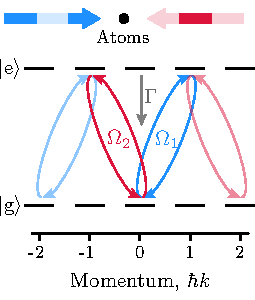
\includegraphics{fig-ai/ssh-scheme.pdf}
    \hfill
    \addletter{140}{b}
    \includegraphics{fig-py/ssh-model.pdf}
    \caption{
        \textbf{Momentum-space dynamics in the SSH model}. 
        a) Atoms undergo momentum-changing transitions via couplings $\Omega_1$ and $\Omega_2$, realizing a SSH-like quantum walk.
        b) Momentum distributions over time for different beam configurations: single beam (left) shows small shift; two continuous beams (middle) result in fast spreading; alternating beams (right) suppress spread.
    }
    \label{fig:sshmodel}
\end{figure}











\subsection{Image Processing}
На каждой из фотографий в каждой выделенной области хочется уметь отличать наличие атома от его отсутствия, что в контексте наличия шумов становится нетривиальным. Можно было бы просто посчитать Pixel Integral \red{(добавить рисунок, а)}, но можно лучше. Расположим оптику (схема оптики) таким образом, что в среднем на пиксель приходилось по фотону. \red{Измерим} какой сигнал на один фотон мы ожидаем и в соответсвии с этим выставим threshold. Таким образом может быть отфильтрована большая часть шума \red{(b)}. Но дальше можно воспользоваться информацией о том, что атомы излучают кучно \red{(пример двух фото с одним counts, с атомом и без)}, в отличие от случайного шума. Так что отфильтровав низкие частоты, свернув изображение с гауссовым фильтром, пролучаем \red{(c)}. 


















\section{Tweezer Array}

\subsection{Experimental setup}
\red{Здесь схема оптики для подготовки лучей твизеров, схема подключения и генерации}.



\begin{figure}
    \centering
    \addletter{195}{a} \phantom{4}
    \includegraphics[width=0.4\textwidth]{fig-ai/flashing-distribution-scheme.pdf}
    \hspace{10 mm} 
    \addletter{195}{b} \phantom{4}
    \includegraphics[width=0.4\textwidth]{imgs/flashing-distribution-img.jpg}

    \addletter{90}{c}
    \includegraphics{fig-py/flashing-oscilloscope.pdf}

    \caption{
        \textbf{Distribution board for flashing}. 
        a) Optical layout of the board used to combine and control light for free-space imaging states $\ket{3}$ and $\ket{6}$.
        b) Experimental implementation.
        c) PD signal of the flashing measured on an oscilloscope (black -- a single experimental run, blue -- the standard deviation over 20 runs, red -- rise time).
    }
    \label{fig:flashing}
\end{figure}



\subsection{Generating with AODs}
% !TEX root = ../master-thesis.tex

\begin{figure}
    \centering
    \includegraphics{fig-ai/preparation-seq.pdf}
    \caption{
        \textbf{Experimental sequence for deterministic atom number preparation.} 
        After loading a spin-balanced mixture into a crossed ODT from the MOT, we perform two-stage evaporation in the ODT. The atoms are then transferred into an optical tweezer via an adiabatic ramp. Further evaporation is carried out in the tweezer before executing the spilling procedure. Spilling takes place at 527\,G and a magnetic field gradient of 20\,G/cm to remove atoms above the spill level. The full sequence enables high-fidelity few-body preparation within a sub-2\,s cycle time. A detailed description can be found in~\cite{culemann_construction_2024}.
    }
    \label{fig:preparationseq}
\end{figure}


% \textbf{Acousto Optic Deflector (AOD)}. AOD, как и AOM, состоит из кристалла, который модулируется пьезоэлементом. Проходящие через кристалл фотоны $(\sub{\vc{k}}{in}, \sub{\omega}{in})$ рассеиваются на фононах $(\vc{q}, \Omega)$ via Bragg diffraction. To have higher efficiency we need to satisfy Bragg condition (проверить и добавить источник)
% \begin{equation*}
% 	\sub{n}{sc} q = \sub{k}{in} \sin(\theta),
% \end{equation*}
% \grey{где $\theta$ это угол между $\vc{k}$ и нормалью к $\vc{q}$} \red{(добавить рисунок)}. Внутри AOD находится несколько пьезоэлементов, к которым ведут провода подобранной длины так, чтобы при изменение частоты $\Omega$ направление $\vc{q}$ менялось соответсвующим Bragg condition образом. Это помогает улучшить диффракционную эффективность \grey{(добавить определение или ссылку)} AOD. На выходе полуются $(\sub{\vc{k}}{out}, \sub{\omega}{out}) = (\sub{\vc{k}}{in}+\vc{q}, \sub{\omega}{in} + \Omega)$. 
% Имея набор частот в модулирующем сигнале $(\vc{q}_j, \Omega_j)$ получим на выходе набор лучей
% \begin{equation*}
% 	(p_j, \vc{k}_j, \omega_j) = (F_j(\vc{a}, \sub{\vc{\omega}}{in}), \sub{\vc{k}}{in}+\vc{q}_j, \sub{\omega}{in} + \Omega_j),
% \end{equation*}
% c мощностью в каждом луче на выходе $p_j$. Регулируя вектор амплитуд $\vc{a}$, подающихся в AOD можно контролировать выходную мощность $\vc{p}$. 



\textbf{Beam collimation and polarization.} The tweezer array is formed by delivering light from a fiber outcoupler and collimating it with an $f = 40\,\mathrm{mm}$ achromatic lens mounted on a translation stage for precise control. To ensure efficient diffraction through the acousto-optic deflectors (AODs), horizontal polarization is set using a $\lambda/2$ waveplate and a polarizing beam splitter (PBS). Correct alignment of the PBS is verified by tracking the beam position on a camera before and after insertion.

\textbf{Acousto-optic deflectors and relay imaging.} The array is generated using a pair of orthogonally mounted AODs, each mounted on custom blocks to maintain a common beam height of 100\,mm. The beam is guided into the first AOD using two mirrors, and its alignment is optimized to maximize both transmission and diffraction efficiency (typically exceeding 90\% at 65\,MHz). The two AODs are connected via a 4f relay built from achromatic lenses in a 30\,mm cage system. Precise positioning is achieved by aligning the relay externally using collimated light and checking for minimal wavefront distortion on a shear plate. An iris at the Fourier plane of the relay filters out the zeroth diffraction order.

\textbf{Telescope and beam expansion.} After the second AOD, the beam is expanded using a telescope consisting of $f = 150\,\mathrm{mm}$ and $f = 500\,\mathrm{mm}$ lenses. The alignment ensures that the beam is collimated and centered on both lenses. The position of the second lens is mechanically fixed, while the telescope length is adjusted via mirror positions to achieve good collimation, verified with a shear plate. The zeroth-order beam after the second AOD is blocked at the intermediate focus.

\textbf{Monitoring and power balancing.} A flip mirror is installed in the beam path to optionally redirect the light into a monitoring camera without disturbing the main optical alignment. This enables fast access to the tweezer array profile during alignment or balancing procedures.

We avoid using a back-side polished mirror for beam sampling in front of the camera. Although commonly employed for its simplicity, such mirrors introduce (\red{? add measured data: october 2024}) spatially varying interference fringes due to reflections from different internal surfaces of the substrate. These fringes distort the measured intensity distribution, especially for rays entering the camera at different angles and positions. This effect becomes critical when calibrating the response of the AODs, as it leads to systematic errors in measured beam uniformity. Instead, we sample the beam with a removable flip mirror that fully redirects the beam, ensuring an undistorted and angle-independent intensity profile at the camera plane.


\subsection{Control}
% !TEX root = ../master-thesis.tex

\textbf{Frequency to position mapping.}
To extract the local intensities $P_{ij}$ from camera images, we need to determine which pixels correspond to which tweezer sites. For this purpose, we define an affine transformation from the drive frequency space $(\omega_{\mathrm{hor}}, \omega_{\mathrm{ver}})$ to image plane coordinates $(x, y)$:
\begin{equation*}
    \vc{r} = H \vc{\omega},
    \hspace{5 mm} \Leftrightarrow \hspace{5 mm} 
    \begin{pmatrix}
        x \\ y
    \end{pmatrix} = \begin{pmatrix}
        h_{11} & h_{12} & h_{13} \\
        h_{21} & h_{22} & h_{23}
    \end{pmatrix} 
    \begin{pmatrix}
        \sub{\omega}{hor} \\
        \sub{\omega}{ver} \\
        1
    \end{pmatrix}.
\end{equation*}
Here, $H$ is a $2 \times 3$ matrix calibrated from a set of measured spot positions. For example, one can measure $\vc{r}_j$ for random frequency vectors $\vc{\omega}_j \in [\omega_{\mathrm{min}},\, \omega_{\mathrm{max}}]$, construct the matrices $\omega_{ij}$ with $i \in \{\mathrm{hor}, \mathrm{ver}\}$ and $r_{ij}$ with $i \in \{x, y\}$, and solve the least-squares problem:
\begin{equation}
    r = H \omega,
    \hspace{0.5cm} \Rightarrow \hspace{0.5cm}
    r \omega^\mathrm{T} = H \omega \omega^\mathrm{T}
    \hspace{0.5cm} \Rightarrow \hspace{0.5cm}
    r \omega^\mathrm{T} \left(\omega \omega^\mathrm{T}\right)^{-1} = H.
    \label{eq:linreg-freq2pos}
\end{equation}

This transformation defines a region of interest around each tweezer, within which we compute the integrated pixel intensity after background subtraction. The resulting values are proportional to the optical powers $P_{ij}$.

\textbf{Linear reconstruction.}
The mapping from input amplitudes $\vc{a}$ to optical power is approximated by Eq.~\eqref{eq:taylerexp}. In the regime $a_i \in [0.85, 0.95]$, a linear approximation is sufficient\footnote{
    For wider amplitude ranges, higher-order terms can be added to the model. However, this is unnecessary in the present context.
}. We construct the Jacobian matrix $F'_{ji}$ by fitting a linear regression model to a dataset of amplitude–intensity pairs. The resulting crosstalk matrix is shown in Fig.~\ref{fig:control}b. It is approximately diagonal, with comparable diagonal entries and off-diagonal elements typically reaching up to 30\% in magnitude relative to the diagonal, due to power redistribution between neighboring tones. Crosstalk between the horizontal and vertical AODs remains negligible.

The quality of the linear fit for the $4 \times 4$ array is illustrated in Fig.~\ref{fig:control}e. The total intensity (Fig.~\ref{fig:control}d) scales linearly with the average input amplitude, yielding $R^2 > 0.99$. Relative residuals are normally distributed with width $0.3\%$, confirming the applicability of the model in this range.

\textbf{Power-aware optimization.}
\grey{In the presence of limited laser power and finite AOM diffraction efficiency, we prefer solutions where all amplitudes remain close to 1. This preference can be incorporated into the optimization objective. In addition to minimizing intensity imbalance, we penalize deviations of the average amplitudes from a target value (e.g., 0.9).}


\subsection{Balancing}
% !TEX root = ../master-thesis.tex




Precise control over the depth of each optical tweezer is essential for preparing few-fermion systems via spilling techniques. In our setup, each tweezer is initially loaded with approximately \red{100} atoms, which are then selectively removed by ramping down the potential depth. The number of remaining atoms as a function of spill power $x_{\mathrm{sp}}$ exhibits a quantized staircase structure, reflecting the discrete energy levels of the 1D harmonic oscillator. This behavior can be characterized by a step plot~\cite{holten_pauli_2022}.

% \textbf{Step plot.}
To characterize this behavior in our tweezer array, we measure step plots for all sites simultaneously. Figure~\ref{fig:stepplot}a shows the result for a $4 \times 4$ array. For each value of $x_{\mathrm{sp}}$, we acquire 70 experimental realizations and compute the average photon signal per site. 
% This signal serves as a robust proxy for atom number. In contrast to single-atom counting, this approach is parameter-free and effective even for large initial occupancies.
% \textbf{Uniformity characterization.}
To quantify depth inhomogeneity across the array, we fit each step trace with a sigmoid function:
\begin{equation*}
    \sigmoid(x) = \frac{A_j}{1 + \exp\left(-(x - x_j)/\sigma_j\right)},
\end{equation*}
where $x_j$ denotes the center of the step and $\sigma_j$ its width for tweezer $j$. We define a relative uniformity metric as $\std(x_j) / \langle x_j \rangle$. After camera-based balancing (Sec.~\ref{subsec:control}), this metric typically yields $\sim 3\%$, which is insufficient for deterministic preparation across the array. A more precise balancing procedure is therefore required.




% \textbf{Single-value feedback.}
To further improve uniformity, we apply an iterative atom-based feedback scheme. Rather than fitting full step plots, we operate at a single point on the slope of the transition, near the half-filling level $A_j / 2$. At this point, the sigmoid can be approximated by a linear response:
\begin{equation*}
    \sigmoid(x) \approx \frac{A_j}{4 \sigma_j} x - \frac{A_j x_j}{4 \sigma_j},
\end{equation*}
assuming $x_j \gg \sigma_j$.  In the feedback loop, we do not use the fitted sigmoid parameters directly. Instead, we measure a single photon-count matrix $M_{ij}$ and treat it as a linear proxy for the power matrix $P_{ij}$. Since the sigmoid offset $\mathrm{shift} = A_j x_j / (4 \sigma_j)$ is known from the fits, we approximate:
\begin{equation}
    \label{mp-propto}
    M_{ij} + \mathrm{shift} \propto P_{ij} = \Lambda H_i V_j.
\end{equation}
We then factorize this matrix using the method introduced in \eqref{uv-decomposition} and update the amplitudes according to:
\begin{equation*}
    h \rightarrow h + \gamma (H - H_0), \qquad
    v \rightarrow v + \gamma (V - V_0),
\end{equation*}
where $(H_0, V_0)$ is the target point, and $\gamma$ is the feedback rate. This model-free procedure avoids full sigmoid fitting and operates directly on experimental measurements.

Figure~\ref{fig:stepplot}b shows the result of applying this single-value feedback (SVF) protocol to a $4 \times 4$ array. After five iterations, the relative deviation of the fitted step centers is reduced to $0.7(2)\%$, well within the plateau width (typically $\pm5\%$), enabling deterministic state preparation across the full array.
Figure~\ref{fig:svf}a shows the process of applying the SVF protocol to a $6 \times 6$ array. The proportionality coefficient in \eqref{mp-propto} is $A/4\sigma \sim 10(1)$ (the average value is chosen for the plot) for our experiment.




\begin{figure}
    \centering
    \addletter{170}{a}
    \includegraphics{fig-py/svf-avg.pdf}
    \addletter{170}{b}
    \includegraphics{fig-py/svf.pdf}
    \caption{
        \textbf{Single-value feedback (SVF) optimization for a $6 \times 6$ tweezer array.}
        (a) Relative deviation of effective powers $P_j$ across the array during successive SVF steps, quantified as $\mathrm{std}(P_j)/\langle P_j \rangle$. The initial point corresponds to camera-based balancing; subsequent iterations apply SVF with feedback rates $\gamma = 1/20$ and $\gamma = 1/40$. Further iterations did not yield statistically significant improvements. 
        (b) Retrieved horizontal powers $H_i$ and vertical powers $V_j$ (top and third rows), along with corresponding deviations of driving amplitudes from their final target values, $h - h^*$ and $v - v^*$. The recovered $H$, $V$ vectors are extracted from the photon count matrix $M_{ij}$ using factorization as described in \eqref{uv-decomposition}.
    }
    \label{fig:svf}
\end{figure}

\subsection{State preparation}
% !TEX root = ../master-thesis.tex


% \textbf{Tweezer loading.} 
We begin by preparing a spin-balanced mixture in the two lowest hyperfine states, $|1\rangle$ and $|2\rangle$, using a compressed magneto-optical trap (MOT). The atoms are initially loaded into a crossed ODT, where we perform evaporative cooling. This follows closely the sequence described in~\cite{culemann_construction_2024}.

After cooling, the atoms are transferred into a tightly focused optical tweezer potential. The loading process relies on the so-called \emph{dimple trick}~\cite{zurn_few-fermion_2012}, where a tightly confined but deep tweezer potential is superimposed onto the wider ODT reservoir. Because the tweezer affects only a small region of the total cloud, the global temperature $T$ remains approximately unchanged, while the local chemical potential is enhanced. In this regime, the average occupation number $\bar{n}(E_i)$ of a single-particle state $i$ with energy $E_i$ follows the Fermi-Dirac distribution:
\begin{equation}
    \bar{n}(E_i) = \frac{1}{e^{(E_i - \mu)/k_B T} + 1}.
\end{equation}
If the energy gap between the ground state $E_0$ and the Fermi energy $E_F$ is increased such that $(E_0 - E_F) / k_B \gg T$, then $\bar{n}(E_0) \rightarrow 1$. This ensures near-unity occupation of the lowest level, which provides an ideal starting point for deterministic preparation. In our experiment, this condition is achieved by ramping on the tweezer adiabatically while continuing evaporation inside the tweezer. The full loading and cooling sequence is depicted in Fig.~\ref{fig:preparationseq}.

% \textbf{Deterministic few-body preparation via spilling.} 
To isolate a well-defined number of atoms in the lowest motional states of the tweezer, we use the \emph{spilling technique}, as described in~\cite{zurn_few-fermion_2012, holten_pauli_2022}. This method relies on tilting the potential with a magnetic field gradient and reducing the trap depth to allow atoms above a threshold energy to tunnel out. 
The resulting states are shown in Fig.~\ref{fig:preparation}.
% The energy levels and wavefunctions of the effective 1D potential under combined optical and magnetic fields were obtained numerically using a finite-difference method and the Thomas algorithm.

The spilling sequence is performed at a magnetic field of 527\,G, where the two spin states are nearly non-interacting. A magnetic field gradient of 20\,G/cm creates a linear tilt, and the tweezer power is lowered to a value that sets the spill threshold. After a short tunneling time, the trap depth is ramped back up to recapture the remaining atoms. By empirically optimizing these parameters, we achieve deterministic preparation of two atoms per tweezer with a fidelity of 90\,\%. This sequence results in high-fidelity preparation within a total experimental cycle time of less than 2\,s.



\begin{figure}
    \centering
    \includegraphics{fig-py/step-plot-2d.pdf}
    \caption[2D step plot]{
        \textbf{2D step plot.}
        Measured 2D step plot as a function of tweezer power and magnetic field gradient. Each point indicates the average atom number obtained for a given combination of parameters. This map confirms that for any spill power, a suitable magnetic gradient can be found to achieve a desired quantized atom number.
    }
    \label{fig:spillingadd-2d}
\end{figure}





\section{Fermi-Hubbard Model}

\subsection{Introduction}
% !TEX root = ../master-thesis.tex

% --------------------------------------------------------------------------------------
% Intro
% --------------------------------------------------------------------------------------

% \textbf{Overview.}
Understanding the dynamics of isolated quantum systems remains one of the central goals of contemporary many-body physics. Over the last decades, considerable progress has been made in classifying and probing different dynamical regimes, from thermalizing phases consistent with conventional statistical mechanics to exotic non-ergodic phases that violate the Eigenstate Thermalization Hypothesis (ETH). Among these, the Fermi-Hubbard model has emerged as a paradigmatic platform for studying the interplay of interactions, quantum statistics, and disorder in strongly correlated systems.

In the clean, disorder-free limit, the Fermi-Hubbard model exhibits rich equilibrium physics, including Mott insulators, spin ordering, and pseudogap phenomena relevant to high-temperature superconductivity \cite{esslinger_fermi-hubbard_2010}. However, the model also serves as a fertile ground for exploring nonequilibrium phenomena, such as quantum quenches, relaxation, transport, and entanglement dynamics — especially when generalized to include disorder or spatial inhomogeneities.

Recently, theoretical and experimental attention has increasingly shifted toward the role of disorder in quantum many-body dynamics. It is now understood that disorder can lead to fundamentally different behaviors depending on the presence or absence of interactions. For instance:
\begin{itemize}
	\item In the absence of interactions, disorder induces \textit{Anderson localization}, which prevents particle diffusion and leads to persistent memory of initial conditions \cite{anderson_absence_1958}.
	\item When interactions are present, the system may enter the regime of \textit{many-body localization (MBL)}, characterized by the absence of thermalization and slow unbounded entanglement growth \cite{basko_metalinsulator_2006,nandkishore_many-body_2015}.
	% , and emergent local integrals of motion
	\item In contrast, when disorder is weak or absent, the system typically evolves toward local thermal equilibrium, consistent with the predictions of \textit{ETH} \cite{deutsch_quantum_1991,srednicki_chaos_1994}. 
\end{itemize}

These dynamical phases — \emph{thermal, Anderson-localized, and MBL} — are typically distinguished through the behavior of local observables, spectral statistics, and the dynamics of quantum correlations. Their interplay is especially rich in two dimensions, where the presence of more complex geometry, potential mobility edges, and rare-region effects make the dynamical phase diagram both challenging and intriguing.

From an experimental standpoint, studying such phenomena requires precise control over initial states, evolution Hamiltonians, and high-fidelity measurements of observables at the single-site level. This thesis presents a platform that provides such control, combining deterministic initialization of fermionic states in a two-dimensional tweezer array with programmable evolution under the Fermi-Hubbard Hamiltonian and spin- and site-resolved imaging.

Compared to conventional optical lattice experiments, the tweezer-based approach offers several key advantages for nonequilibrium quantum simulation:
\begin{enumerate}
	\item \textit{Deterministic and programmable state preparation.} Using a sequence of global and spin-selective spilling operations, arbitrary configurations of fermionic atoms can be prepared with high fidelity. This capability enables initialization of tailored many-body states for probing specific dynamical scenarios, such as local quenches, domain-wall melting, or imbalance relaxation.
	\item \textit{Fast experimental cycle and large statistics.} The entire experimental sequence, including preparation, evolution, and measurement, completes in under two seconds, allowing up to $10^5$ experimental repetitions per day. This rapid repetition rate is crucial for averaging over disorder realizations and collecting sufficient statistics for dynamical observables.
	\item \textit{Spin- and site-resolved detection.} The developed imaging system supports fluorescence-based, single-shot discrimination of atomic spin states on individual lattice sites. This enables direct access to observables such as density profiles $\langle n_j \rangle$, magnetization $\langle \sigma^z_j \rangle$, and spin correlations $\langle \sigma^z_i \sigma^z_j \rangle$ — all of which are sensitive to the system's dynamical regime.
\end{enumerate}

In tandem with experimental capabilities, in this work a numerical simulation package was developed for modeling real-time dynamics in finite-size Hubbard systems. The package combines exact diagonalization (ED) for small systems and Krylov subspace methods for larger Hilbert spaces (up to $10^9$ dimensions), and supports evaluation of observables and entanglement entropy in arbitrary geometries and disorder realizations.

Together, these tools enable a systematic exploration of the dynamical phase diagram of the disordered Fermi-Hubbard model in two dimensions. By leveraging control over initial conditions, disorder strength, and interactions, as well as the ability to access key observables, one can address central questions in nonequilibrium many-body physics: What determines whether a system thermalizes? When does localization persist in the presence of interactions? How do correlations and entanglement spread in different regimes?

In the following subsections, we review the theoretical framework underpinning these questions, beginning with the concept of thermalization in isolated quantum systems.



\subsection{Code}
...

% А тут расскажу про модель, которую сделал и что мы можем в нашем эксперименте наблюдать. 



% The entanglement entropy between two halves of a $4 \times 4$ Fermi-Hubbard system with $N_\uparrow = N_\downarrow = 2$ is bounded by the logarithm of the Schmidt rank of the reduced density matrix $\rho^A$. Due to particle number conservation, $\rho^A$ decomposes into orthogonal blocks labeled by $(N_\uparrow^{(A)}, N_\downarrow^{(A)}) = (k, l)$. The maximal rank of each block is given by the minimal dimension of the matching sectors in subsystems $A$ and $B$. Thus, the total maximal rank is

% \begin{equation*}
% R_{\max} = \sum_{k=0}^2 \sum_{l=0}^2 \min\left[ \binom{8}{k} \binom{8}{l}, \binom{8}{2-k} \binom{8}{2-l} \right] = 154.
% \end{equation*}

% The corresponding maximal entropy is

% \begin{equation*}
% S_{\max} = \ln(R_{\max}) = \ln(154) \approx 5.04.
% \end{equation*}



\section{Appendix}

% \newpage
% (добавить кликабельные ссылки через href)

Statement of Interest

% intro
Я заинтересован в проведении PhD-исследований в лаборатории IOL, поскольку её направления идеально совпадают с моими научными интересами и навыками: применение ML-методов для решения математических задач (AI4Science), численные методы для моделирования квантовых многочастичных систем, а также подходы на основе выпуклой оптимизации, в частности алгоритмы Франка-Вольфа.

% project I
У меня есть два значимых исследовательских достижения, релевантных для проектов IOL. Первое связано с разработкой метода на основе машинного обучения, который позволил впервые успешно исследовать графы Кэли достаточно большой размерности, что начал собираться кубик Рубика 5x5 (около 10^70 вершин). Этот подход стал state-of-the-art (превзойдя все соответствующие на Kagle решения по средней длине по кубикам 3x3, 4x4, 5x5), и подтвердил перспективность ML-методов в решении задач дискретной оптимизации. Этот опыт непосредственно связан с проектами IOL в области оптимизации, такими как улучшение хроматических оценок плоскостей.

% project II: BMF, FW-alg, model-based control -> !
Второе значимое достижение связано с моей магистерской диссертацией, в рамках которой я разработал набор методов для эффективной подготовки произвольных квантовых состояний с разрешением по положению и спину в решётке для квантовых симуляторов. Предложенные мной протоколы основываются на model-based control. Они включали методы выпуклой оптимизации, обеспечив заселение проивзольных фермионных мод (sit and spin resolved deterministic state preparation) квантовых состояний. Этот опыт особенно близок проекту IOL по использованию алгоритмов Франка-Вольфа. В целом лаборатория в которой работаю, возникла вокруг идеи детекции запутанности, что перекликается с проектом IOL.

% some general experience description
Также у меня имеется опыт численных симуляций квантовых многочастичных систем, таких как эволюция модели Ферми-Хаббарда с помощью методов на основе Крылов-подпространств и построение фазовых диаграмм с помощью алгоритмов DMRG. Я проявляю большой интерес к проектам лаборатории по симуляции открытых квантовых систем и использованию Tensor Networks для моделирования квантовых цепочек и схем. Мой опыт в области GPU-программирования и распараллеленных вычислений будет полезен для дальнейших исследований лаборатории, связанных с высокопроизводительными вычислениями.

% свои идеи
Кроме этого, у меня есть несколько конкретных идей, которые я хотел бы реализовать в рамках PhD в IOL:
Применение методов машинного обучения для направления случайных блужданий по flip-graphs с целью поиска оптимальных или близких к оптимальным схем матричных операций и тензорных разложений.
Развитие подходов, объединяющих достижения FermiNet и Tensor Networks, для моделирования многочастичных фермионных и других сложных квантовых систем.
Разработка алгоритмов и методик для эффективной декомпозиции квантовых схем с использованием подходов MPO, что позволит существенно упростить численные расчёты и реализацию экспериментальных схем.
Создание и тестирование протоколов детекции запутанности с использованием алгоритмов Франка-Вольфа для различных платформ квантовых симуляторов.
Вообще понятно как обучать модель решать кубо задачи. Сначала для х находим непрерывной оптимизацией Q, и так формируем датасет. А затем делаем дистилляцию ошибки. 

- А ещё симметрии это важно. Так они и в оценке чисел Гротендика помогли, и для флип-графов. 
- Хорошо, когда можем легко сгенерировать охапку решений. 
- Здорово, когда можем потихоньку это решение портить и пытаться это откатить.

!!!!!!!!!!!!!!!!
- Для QUBO решение обратной задачи, это уже просто непрерывная оптимизация, что можно делать эффективно. Так что можно для случайного x, эффективно находить Q такое что x = argmax xᵀQx. И теперь можем обучать модель по Q предсказывать x.  
- Да, это не панацея, но мне кажется любопытным направлением. Не нужно предсказывать x сразу, пусть скорее модель предсказывает а какие пиксели в х скорее всего нужно поменять, и затем на её основе делать отжиг или parallel tempering. 
!!!!!!!!!!!!!!!!

% Plans
В долгосрочной перспективе я планирую заниматься исследовательской деятельностью, как в ведущих научных центрах, так и рассматриваю создание собственной исследовательской группы с направлением AI4Science. Мне важно в рамках PhD глубже разобраться в фундаментальных аспектах, приобрести опыт проведения самостоятельных исследований, а также научиться управлять проектами, организовывать совместные исследования и руководить научной группой. Лаборатория IOL является для меня идеальным местом для реализации этих целей, поскольку здесь сосредоточен уникальный опыт в прикладной математике, машинном обучении и численных методах, идеально соответствующий моим амбициям и навыкам.

% call to action
Буду рад возможности обсудить конкретные идеи проектов и начать сотрудничество с вашей лабораторией.




Хочу расти дальше. Закончил ресеарч фазу в этой компании, два продукта готовы. 
Лучше фокусировать на личной мотивации, мне важны задачи, продолжать исследование. 
Есть дополнительные вопросы, больше деталей. Должно быть кристально ясно. В STAR рассказать как есть. 
At the beginning I have this situation. 
My Task. My actions. Больше деталей.
A did this actions.


Ставить точки. 

В качестве development хорошо указывать курсы, конференции.

Про мотивацию давать примеры. 

Hi Dmytro, I saw that you liked my GitHub repo—appreciate it! I’m curious, how did you find it?

Hi Dmytro, I saw that you liked my GitHub repo—appreciate it! I’m curious, how did you find it?

Also I’m looking into quantum circuit decomposition probles, and I’d love to hear what challenges you find most pressing there.

\subsection{Image Processing}
% !TEX root = ../master-thesis.tex

\textbf{From frequency to position}. И в camera based balancing, и в atoms based balancing для обработки изображений удобно определить афинное преобразование из frequency space to position space:
\begin{equation*}
	\vc{r} = H \vc{\omega}
	\hspace{5 mm} \leftrightarrow \hspace{5 mm} 
	\begin{pmatrix}
		x \\ y
	\end{pmatrix} = \begin{pmatrix}
		h_{11} & h_{12} & h_{13} \\
		h_{21} & h_{22} & h_{23} \\
	\end{pmatrix} 
	\begin{pmatrix}
		\sub{\omega}{hor} \\
		\sub{\omega}{ver} \\
		1
	\end{pmatrix}.
\end{equation*}
Можно, например, для случайных $\vc{\omega}_j \in [\sub{\omega}{min},\, \sub{\omega}{max}]$ измерить $\vc{r}_j$, таким образом сформировав две матрицы $\omega_{ij}$ with $i \in \{\mathrm{hor},\, \mathrm{ver}\}$ and $r_{ij}$ with $i \in \{x, y\}$. Остается решить уравнение на $H$ (что соответсвует Least squares method):
\begin{equation}
	r = H \omega,
	\hspace{0.5cm} \Rightarrow \hspace{0.5cm}
	r \omega\T = H \omega \omega\T
	\hspace{0.5cm} \Rightarrow \hspace{0.5cm}
	r \omega\T \left(\omega \omega\T\right)^{-1} = H.
	\label{LinReg:freq2pos}
\end{equation}

\subsection{Boolean Decomposition}
% !TEX root = ../master-thesis.tex

...

% Мы хотим найти разложение булевой матрицы $W_{ij}$ размера $n\times n$
% \begin{equation*}
% 	W_{ij} = \sum_{\lambda=1}^r u^\lambda_i v^\lambda_j,
% \end{equation*}
% для наименьшего булева ранга $r$ (или bipartite dimension). Всевозможных матриц $\card\{W_{ij}\} = 2^{n^2}$. Для $n \leq 5$ it about 34 miilion states, so it can be decomposed with brute force \red{(ссылка на код)}. \grey{Можно }

% Для больших $n$ можем попробовать подход с flip graph. TBA. 



\bibliographystyle{plain}
\bibliography{master-thesis.bib}


\end{document}


